\documentclass[12pt]{article}\usepackage[]{graphicx}\usepackage[]{color}
%% maxwidth is the original width if it is less than linewidth
%% otherwise use linewidth (to make sure the graphics do not exceed the margin)
\makeatletter
\def\maxwidth{ %
  \ifdim\Gin@nat@width>\linewidth
    \linewidth
  \else
    \Gin@nat@width
  \fi
}
\makeatother

\definecolor{fgcolor}{rgb}{0.345, 0.345, 0.345}
\newcommand{\hlnum}[1]{\textcolor[rgb]{0.686,0.059,0.569}{#1}}%
\newcommand{\hlstr}[1]{\textcolor[rgb]{0.192,0.494,0.8}{#1}}%
\newcommand{\hlcom}[1]{\textcolor[rgb]{0.678,0.584,0.686}{\textit{#1}}}%
\newcommand{\hlopt}[1]{\textcolor[rgb]{0,0,0}{#1}}%
\newcommand{\hlstd}[1]{\textcolor[rgb]{0.345,0.345,0.345}{#1}}%
\newcommand{\hlkwa}[1]{\textcolor[rgb]{0.161,0.373,0.58}{\textbf{#1}}}%
\newcommand{\hlkwb}[1]{\textcolor[rgb]{0.69,0.353,0.396}{#1}}%
\newcommand{\hlkwc}[1]{\textcolor[rgb]{0.333,0.667,0.333}{#1}}%
\newcommand{\hlkwd}[1]{\textcolor[rgb]{0.737,0.353,0.396}{\textbf{#1}}}%
\let\hlipl\hlkwb

\usepackage{framed}
\makeatletter
\newenvironment{kframe}{%
 \def\at@end@of@kframe{}%
 \ifinner\ifhmode%
  \def\at@end@of@kframe{\end{minipage}}%
  \begin{minipage}{\columnwidth}%
 \fi\fi%
 \def\FrameCommand##1{\hskip\@totalleftmargin \hskip-\fboxsep
 \colorbox{shadecolor}{##1}\hskip-\fboxsep
     % There is no \\@totalrightmargin, so:
     \hskip-\linewidth \hskip-\@totalleftmargin \hskip\columnwidth}%
 \MakeFramed {\advance\hsize-\width
   \@totalleftmargin\z@ \linewidth\hsize
   \@setminipage}}%
 {\par\unskip\endMakeFramed%
 \at@end@of@kframe}
\makeatother

\definecolor{shadecolor}{rgb}{.97, .97, .97}
\definecolor{messagecolor}{rgb}{0, 0, 0}
\definecolor{warningcolor}{rgb}{1, 0, 1}
\definecolor{errorcolor}{rgb}{1, 0, 0}
\newenvironment{knitrout}{}{} % an empty environment to be redefined in TeX

\usepackage{alltt}

% make wider margins
\usepackage[margin=1in]{geometry}


%%%%%%%%%%%%%%%%%%%%%%%%%%%%%%%%%%%%%%%%%%%%%%%%%%%%%%%%%%%%%%%%
%
% Formatting
%
%%%%%%%%%%%%%%%%%%%%%%%%%%%%%%%%%%%%%%%%%%%%%%%%%%%%%%%%%%%%%%%%
  
% define font
\usepackage{times}

% math symbols
\usepackage{amsmath, amsfonts, amssymb, bbm, bm}

%remove extra space for align environments
\setlength{\abovedisplayskip}{-15pt}
\setlength{\belowdisplayskip}{0pt}
% \newcommand{\zerodisplayskips}{
%   \setlength{\abovedisplayskip}{3pt}
%   \setlength{\belowdisplayskip}{8pt}
%   \setlength{\abovedisplayshortskip}{10pt}
%   \setlength{\belowdisplayshortskip}{10pt}}
% \appto{\normalsize}{\zerodisplayskips}

% extra graphics and figures formatting and options
\usepackage{graphicx,caption,subcaption,rotating,float,rotating,calc,fancyhdr,url,tablefootnote, titlesec,titletoc,arydshln}

% bullet lists, etc. with custom indentation
\usepackage{enumerate}

% easy in-text citations and colored urls
% \usepackage[colorlinks = true,
%             linkcolor = blue,
%             urlcolor  = blue,
%             citecolor = blue,
%             anchorcolor = blue]{hyperref}

% tell latex to not hyphenate words!!!
%\usepackage[none]{hyphenat}

% let equations spill over multiple pages
\allowdisplaybreaks

%line and sentence spacing and page formatting
% \usepackage[tablesfirst,notablist]{endfloat}
\usepackage{setspace,lineno,breakcites}
\usepackage[title]{appendix}


%captions formatting
%\usepackage[small,it]{caption}
%\addtolength{\belowcaptionskip}{-3mm}
%\addtolength{\abovecaptionskip}{-3mm}
%\addtolength{\intextsep}{-3mm}

%bibliography
\usepackage[authoryear]{natbib}
\bibliographystyle{besjournals}

%Miscellaneous formatting for paper
\newcommand*\mystrut[1]{\vrule width0pt height0pt depth#1\relax}
\providecommand{\keywords}[1]{\textbf{Key Words:} #1}
\renewcommand{\refname}{Literature Cited} 

%Define math operators myself
\newcommand\Tau{\mathcal{T}}

%Adding multiple authors with multiple affiliations
\usepackage{authblk}

%Making key words heading
\providecommand{\keywords}[1]{\textbf{Key Words:} #1}

%Remove space before section headers
\titlespacing{\section}{0pt}{0pt}{0pt}



%%%%%%%%%%%%%%%%%%%%%%%%%%%%%%%%%%%%%%%%%%%%%%%%%%%%%%%%%%%%
%%%
%%% Title, Authorship
%%%
%%%%%%%%%%%%%%%%%%%%%%%%%%%%%%%%%%%%%%%%%%%%%%%%%%%%%%%%%%%%

\title{Survival Analaysis Report}

\author[1]{Alison C. Ketz}
\affil[1]{Department of Forest and Wildlife Ecology, University of Wisconsin, Madison, aketz@wisc.edu}
\author[2]{Dan P. Walsh}
\affil[2]{National Wildlife-Health Center, U.S. Geological Survey, Madison, WI}

%%%%%%%%%%%%%%%%%%%%%%%%%%%%%%%%%%%%%%%%%%%%%%%%%%%%%%%%%%%%
%%%
%%% Begin Document
%%%
%%%%%%%%%%%%%%%%%%%%%%%%%%%%%%%%%%%%%%%%%%%%%%%%%%%%%%%%%%%%
\IfFileExists{upquote.sty}{\usepackage{upquote}}{}
\begin{document}
% print document title
\maketitle

\doublespace

%%%%%%%%%%%%%%%%%%%%%%%%%%%%%%%%%%%%%%%%%%%%%%%%%%%%%%%%%%%%
%%%
%%% Load libraries and set up cache
%%%
%%%%%%%%%%%%%%%%%%%%%%%%%%%%%%%%%%%%%%%%%%%%%%%%%%%%%%%%%%%%



%%%%%%%%%%%%%%%%%%%%%%%%%%%%%%%%%%%%%%%%%%%%%%%%%%%%%%%%%%%%
%%%
%%% Title page
%%%
%%%%%%%%%%%%%%%%%%%%%%%%%%%%%%%%%%%%%%%%%%%%%%%%%%%%%%%%%%%%
  
\maketitle
\date


%%%%%%%%%%%%%%%%%%%%%%%%%%%%%%%%%%%%%%%%%%%%%%%%%%%%%%%%%%%%
%%%
%%% Background and Methods
%%%
%%%%%%%%%%%%%%%%%%%%%%%%%%%%%%%%%%%%%%%%%%%%%%%%%%%%%%%%%%%%

\section{Introduction and Methods}

The purpose of this document is to outline the results of the preliminary survival analysis for the WIDNR southwestern deer study from the first year of data available. This analysis uses data from captured and collared adult individuals during the first few months of 2017 to estimate adult survival until the first week of January 2018. It is quite early in this study for such an analysis, so we suggest extreme caution with interpretation of all results.

Survival was estimated with a conditional continuous time to event model, also called a known fate hazard model \citep{kalbfleisch_statistical_2002}. The basic formulation of the likelihood can be found in \citet{walsh_using_2017} and allows for left truncation and interval-censored data. Survival is modeled on a weekly time scale, because it is computationally faster. Future analysis could use a finer time resolution (daily) if deemed necessary. Individuals suriviving to the end of the study period were right truncated at 52 weeks. Capture-induced mortalities were also right censored. A peice-wise cumulative discrete hazard model was used to approximate the unit cumulative hazard model, with a complementary log-log link function. Two models were fit using Bayesian methods and implemented in JAGS \citep{plummer_jags:_2004}, with standard diagnostics indicating no lack of fit. The first model included a discrete covariate for chronic wasting disease (CWD) status (positive or negative at capture or after mortality when available) in the hazard rate function, and a second model included covariates for both disease status and sex of the collared individual. No other covariates were considered at this time, but can be included in future analyses. 

The live RAMALT test for CWD used in this study has been shown to have low sensitivity and high specificity with additional heterogeneities arising from disease stage and the PRNP genotype \citep{thomsen_diagnostic_2012}. In de-populated captive cervid farms in Canada and the US, \citet{thomsen_diagnostic_2012} calculated a pooled sensitivity of the RAMALT test of 68\% with 95\% credible limits of 49 and 82. We incorporated this test sensitivity for the individuals who tested negative for CWD at capture using a zero-inflated bernoulli model. Observed CWD status at capture ($x_1$) is modeled with a Bernoulli distribution that depends on the true disease status at capture and the probability of detecting the disease given that it is actually present, also known as the sensitivity ($p$). The true disease state ($\bm{z}$) was also modeled with a Bernoulli disribution depending on the prevalence ($\psi$) of the disease.
\begin{align}
    x_{1,j} & \sim \text{ Bernoulli }(p *z_j)\\
    z_j & \sim \text{ Bernoulli }(\psi)\\
    p & \sim \text{ beta }(92.5,44.5)\\
    \psi & \sim \text{ uniform }(0,1),
\end{align}

\noindent for $j$ in $1,...,J$ records. A flat uniform (0,1) prior distribution was specified for prevalence ($\psi$). The parameters in the informed prior beta distribution of sensitivity ($p$) were moment matched \citep{hobbs_bayesian_2015} from the pooled estimate of sensitivity from \citet{thomsen_diagnostic_2012}. Flat normal prior distributions were used for the coefficients in the hazard rate model.


%%%%%%%%%%%%%%%%%%%%%%%%%%%%%%%%%%%%%%%%%%%%%%%%%%%%%%%%%%%%
%%%
%%% Results
%%%
%%%%%%%%%%%%%%%%%%%%%%%%%%%%%%%%%%%%%%%%%%%%%%%%%%%%%%%%%%%%

\section{Results}

Posterior distributions of the coefficients in the hazard rate models were calculated for both models. The baseline intercept for the analysis represents the hazard for CWD negative individuals for the first model, and CWD negative females for the second model. Other states were represented with the additive coefficient terms in the hazard rate model.

% latex table generated in R 3.4.2 by xtable 1.8-2 package
% Mon Jan  8 15:18:57 2018
\begin{table}[H]
\centering
\caption{Coefficients of the hazard rate analysis where the baseline hazard shows the hazard for chronic wasting disease negative adult individuals not exposed to harvest, with additive hazard effects in the following three rows. The first column denotes the mean of the posterior distribution with the standard deviation (SD), and equal-tailed Bayesian credible intervals in the right two columns.} 
\label{tab:hazard_v7}
\begin{tabular}{ccccc}
 Coefficient & Mean & SD & .025 & .975 \\ 
  \hline
CWD(-), No harvest & -5.91 & 0.3 & -6.53 & -5.36 \\ 
  CWD(+), No harvest & 1.8 & 0.5 & 0.79 & 2.74 \\ 
  Bow Harvest & 0.89 & 0.37 & 0.17 & 1.61 \\ 
  Gun Harvest & 1.07 & 0.43 & 0.19 & 1.89 \\ 
   \hline
\end{tabular}
\end{table}




% latex table generated in R 3.4.2 by xtable 1.8-2 package
% Mon Jan  8 15:18:58 2018
\begin{table}[H]
\centering
\caption{Coefficients of the hazard rate analysis where the baseline hazard shows the hazard for chronic wasting disease positive adult females not exposed to harvest, with additive hazard effects in the following rows. The first column denotes the mean of the posterior distribution with the standard deviation (SD), and equal-tailed Bayesian credible intervals in the right two columns.} 
\label{tab:hazard_v8}
\begin{tabular}{ccccc}
 Coefficient & Mean & SD & .025 & .975 \\ 
  \hline
CWD(-), No Harvest & -6.04 & 0.34 & -6.73 & -5.41 \\ 
  CWD(+), No Harvest & 1.8 & 0.5 & 0.78 & 2.76 \\ 
  Bow Harvest & 0.97 & 0.37 & 0.25 & 1.69 \\ 
  Gun Harvest & 1.06 & 0.43 & 0.18 & 1.89 \\ 
  Sex & 0.08 & 0.34 & -0.59 & 0.75 \\ 
   \hline
\end{tabular}
\end{table}



The intercept term for both models was quite low on the log scale, suggesting relatively low mortality. This is consistent with other white-tailed deer populations and for ungulates in general \citep{gaillard_population_1998}. Chronic wasting disease substantially increased the hazard in both models (Tables 1 and 2). 

Cumulative survival probabilities across all weeks of the study were derived using the posterior values of the hazard rate coefficients. For the first model, including only CWD status, the probability of surviving to the end of the study given exposure to both archery and gun harvest seasons was quite different for the CWD positive individuals than for CWD negative individuals.

The pre-harvest survival period spans from the beginning of the study in January through September 15. The archery and bow season begins September 16 and is ongoing through the rest of the study. The estimated survival probability of archery and bow hunter harvest for the initial bow/archery hunting season were reported in the table as ``Post Bow/Archery", even though this type of harvest could occur throughout the remaining weeks of the study. This cumulative probability was included because all mortalities arising from archery and bow ocurred before the first gun hunting season began. 

Note that none of these survival probabilities are conditional on surviving harvest given that an individual survives to the beginning of each harvest season. The survival probabilities in Tables 3 and 4 and Figures 1 and 2 are cumulative from the origin of the study until the end of the period they denote. For example, the reported survival probability of a CWD negative adult female in Table 4 under the row denoted "Post Gun 1" is not the probability of surviving gun harvest, it is the probability of surviving since the origin of the study including exposure to archery and bow hunting, as well as gun hunting during the initial gun season. The cumulative nature of these survival probabilities are more easily seen in the Figures 1 and 2. The tables are meant to provide a numerical reference, although viewing the tables alone may be confusing. 

\vspace{1 cm}


% latex table generated in R 3.4.2 by xtable 1.8-2 package
% Mon Jan  8 15:18:58 2018
\begin{table}[H]
\centering
\caption{The summary statistics for the posterior distributions of the cumulative probability of survival to the end of several harvest (and non harvest) seasons. The cumulative survival probabilites for archery/bow harvest season are only for the season prior to gun harvest dates. The gun harvest survival probabilities include exposure to bow hunting, however, only gun attributed mortalities occured during those seasons. The right two columns denote the 95\% Bayesian credible intervals.} 
\label{tab:survival_v7}
\begin{tabular}{cccccc}
 Period & CWD Status & Mean & SD & 0.025 & 0.975 \\ 
  \hline
\hline
Pre-Harvest & Negative & 0.91 & 0.03 & 0.85 & 0.95 \\ 
   & Positive & 0.55 & 0.13 & 0.28 & 0.79 \\ 
   \hdashline 
Bow/Archery & Negative & 0.85 & 0.03 & 0.79 & 0.91 \\ 
   & Positive & 0.39 & 0.14 & 0.14 & 0.67 \\ 
   \hdashline 
Gun & Negative & 0.80 & 0.04 & 0.72 & 0.87 \\ 
   & Positive & 0.28 & 0.14 & 0.06 & 0.57 \\ 
   \hdashline 
Holiday Gun & Negative & 0.76 & 0.04 & 0.68 & 0.84 \\ 
   & Positive & 0.21 & 0.13 & 0.03 & 0.51 \\ 
   \hline
\hline
\end{tabular}
\end{table}





\begin{figure}[H]
\begin{center}
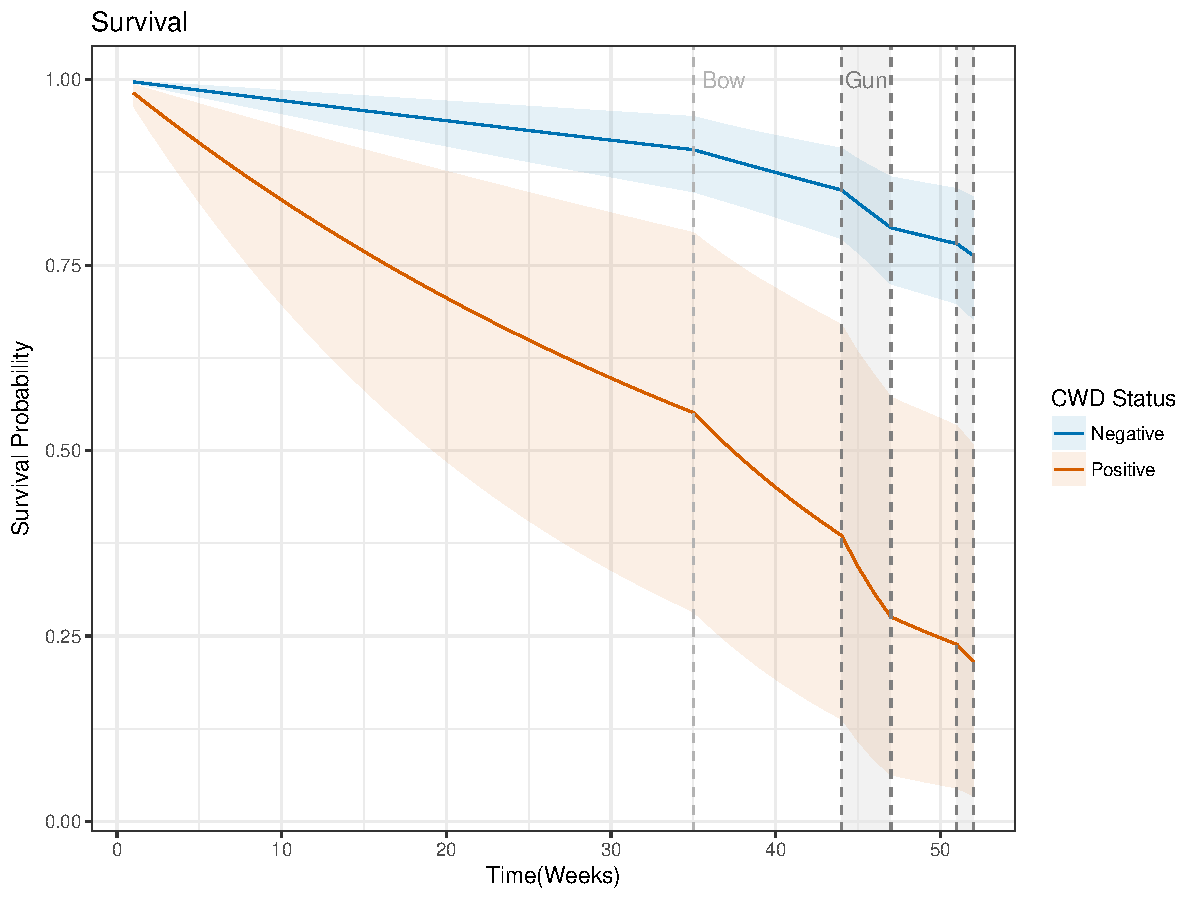
\includegraphics[width=6 in]{figures/Survival_v7}
\caption{The cumulative weekly probability of surviving from the beginning of the study through the end of the first year for chronic wasting disease negative white-tailed deer, for adult females (blue line) and adult males (orange line). The cumulative weekly survival probability for chronic wasting disease positive deer are lower than for negative deer, for both adult females (pink line) and adult males (solid grey line). Equal-tailed 95\% Bayesian credible intervals are shown in the corresponding color shaded regions. The bow hunt harvest season begins at the light grey dashed line and continues to the end of the study. The light grey shaded regions with darker grey dashed lines denote the gun harvest seasons.}\label{fig:survival_v7}
\end{center}
\end{figure}


\begin{figure}[H]
\begin{center}
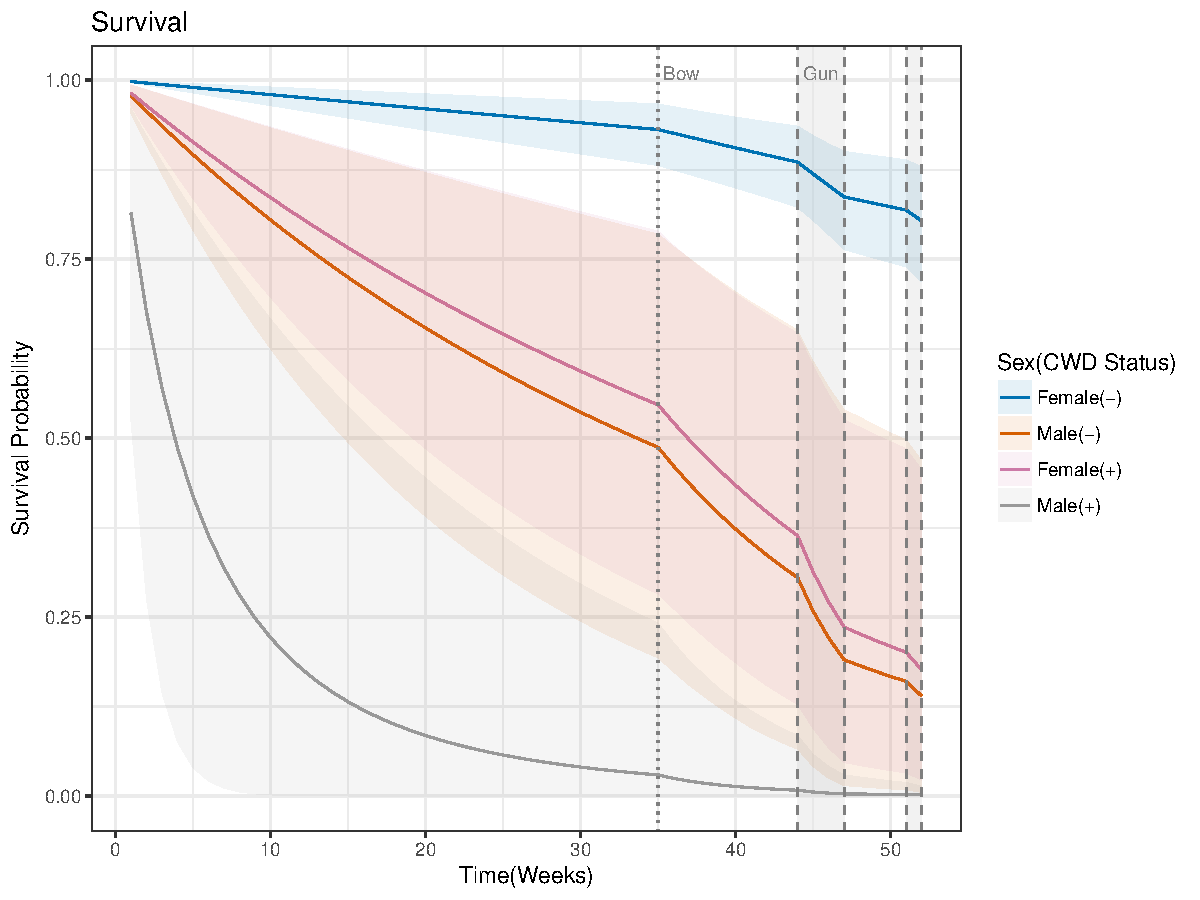
\includegraphics[width=6 in]{figures/Survival_v8_sex}
\caption{The cumulative weekly probability of surviving from the beginning of the study through the end of the first year for chronic wasting disease negative white-tailed deer, for adult females (blue line) and adult males (orange line). The cumulative weekly survival probability for chronic wasting disease positive deer are lower than for negative deer, for both adult females (pink line) and adult males (solid grey line). Equal-tailed 95 \% Bayesian credible intervals are shown in the corresponding color shaded regions. The bow hunt harvest season begins at the light grey dotted line and continues to the end of the study. The light grey shaded regions with darker grey dashed lines denote the gun harvest seasons.}\label{fig:survival_v8}
\end{center}
\end{figure}


% latex table generated in R 3.4.2 by xtable 1.8-2 package
% Mon Jan  8 15:18:58 2018
\begin{table}[H]
\centering
\caption{The summary statistics for the posterior distributions of the cumulative probability of survival to the end of several harvest (and non harvest) seasons. The pre-harvest survival period spans from the beginning of the study through the Septmeber 15. While the archery and bow season continues throughout the study after the middle of September, the probability of survival due to bow and archery harvest alone are reported in the rows denoted bow hunt. The gun harvest survival probabilities include exposure to bow hunting, however only gun attributed mortalities occured during those seasons. The right two columns denote the 95\% Bayesian credible intervals.} 
\label{tab:survival_v8}
\begin{tabular}{ccccccc}
 Period & CWD Status & Sex & Mean & SD & 0.025 & 0.975 \\ 
  \hline
\hline
Pre-Harvest & Negative & Female & 0.92 & 0.03 & 0.85 & 0.96 \\ 
   &  & Male & 0.91 & 0.03 & 0.84 & 0.96 \\ 
   \hdashline 
 & Positive & Female & 0.59 & 0.15 & 0.28 & 0.84 \\ 
   &  & Male & 0.57 & 0.13 & 0.29 & 0.81 \\ 
   \hline
Post Bow/Archery  & Negative & Female & 0.86 & 0.03 & 0.79 & 0.92 \\ 
   &  & Male & 0.85 & 0.04 & 0.76 & 0.92 \\ 
   \hdashline 
 & Positive & Female & 0.42 & 0.16 & 0.12 & 0.72 \\ 
   &  & Male & 0.39 & 0.14 & 0.14 & 0.68 \\ 
   \hline
Post Gun 1 & Negative & Female & 0.81 & 0.04 & 0.72 & 0.89 \\ 
   &  & Male & 0.80 & 0.05 & 0.69 & 0.89 \\ 
   \hdashline 
 & Positive & Female & 0.31 & 0.16 & 0.05 & 0.64 \\ 
   &  & Male & 0.28 & 0.14 & 0.06 & 0.57 \\ 
   \hline
Post Gun 2 & Negative & Female & 0.78 & 0.05 & 0.68 & 0.87 \\ 
   &  & Male & 0.76 & 0.06 & 0.64 & 0.86 \\ 
   \hdashline 
 & Positive & Female & 0.24 & 0.15 & 0.03 & 0.57 \\ 
   &  & Male & 0.21 & 0.13 & 0.03 & 0.51 \\ 
   \hline
\hline
\end{tabular}
\end{table}


As expected, survival decreases throughout the study, and there were large differences between the CWD positive and negative groups. Figure 2 shows survival decomposed by both sex and CWD status. The credible interval of CWD status stops overlapping when harvest begins. Survival curves of both sexes were very similar to one another given CWD status. The sex effect for the hazard rate was small in magnitude, with a credible interval that overlaps zero, suggesting little to no effect. However, all of these estimates are based on a small sample size for only a limited time scale, and consequently, they should be very cautiously interpreted.

\begin{figure}[H]
\begin{center}
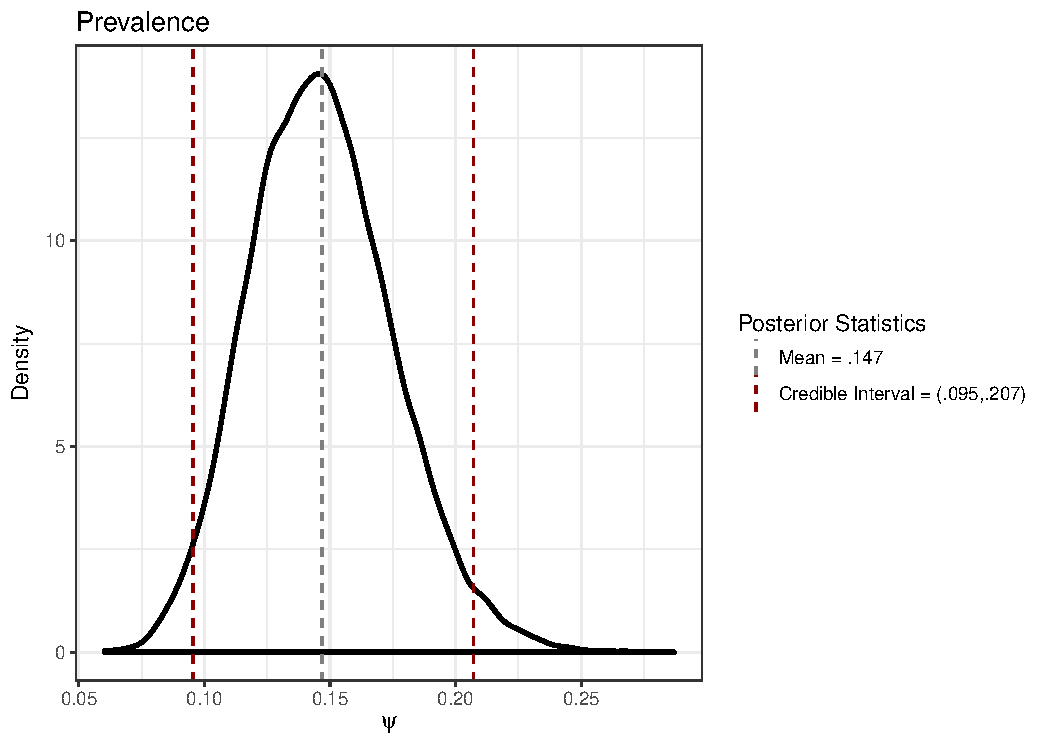
\includegraphics[width=6 in]{figures/Prevalence}
\caption{The posterior distribution of prevalence of chronic wasting disease ($\psi$) obtained from the zero-inflated binomial model of observed CWD status. The mean of the posterior was 0.147 (grey dashed line) with an equal-tailed 95\% Bayesian credible interval of (0.095,0.207) (red dashed lines).}\label{fig:Prevalence}
\end{center}
\end{figure}

Incorporating the sensitivity of the RAMALT test only slightly increased the uncertainty of the posterior distributions. The standard deviations of the posterior distributions of all paramaters increased a small amount, as did the Bayesian credible intervals, but the means of the posteriors were pretty much identical to the results when sensitivity was ignored (not shown). The mean and credible intervals for prevalence of CWD were estimated as 0.147 (0.095,0.207), and were identical for both models (Figure \ref{fig:Prevalence}).

Further work will include a cause-specific survival analysis of adults and a survival analysis of fawns. As sample sizes increase, we can also increase the resolution of the time-step to daily.


%%%%%%%%%%%%%%%%%%%%%%%%%%%%%%%%%%%%%%%%%%%%%%%%%%%%%%%%%%%%
%%%
%%% References
%%%
%%%%%%%%%%%%%%%%%%%%%%%%%%%%%%%%%%%%%%%%%%%%%%%%%%%%%%%%%%%%
\singlespacing
\bibliography{survival}
% \printbibliography


\end{document}





